\documentclass{sig-alternate-10pt}
\usepackage{amsfonts,xspace}
\usepackage{url}
\usepackage{epsfig}
\usepackage{graphicx}
\usepackage{subfigure}
\usepackage{ifpdf}
\usepackage[usenames,dvipsnames]{color}
\newcommand{\tbd}[1]{}
\newcommand{\ie}{{\it i.e.}}
\newcommand{\eg}{{\it e.g.}}
\newcommand{\etc}{{\it etc.}}
\newcommand{\eat}[1]{}
\usepackage[english,plain]{fancyref}
\usepackage{times}
\usepackage{rotating}
\usepackage[labelformat=simple]{subfig}


\newcommand{\mypara}[1]{\medskip\noindent{\bf {#1}:}~}
\newcommand{\chk}{$\checkmark$}
\newcommand{\dsh}{{\bf --}}
\newcommand{\til}{{\bf\large \textasciitilde}}
%\newcommand{\tbd}[1]{[{\color{red}{\bf{TBD: #1}}}]}
\newcommand{\etal}{\emph{et~al.}}
\newcommand{\meddle}{{Meddle}\xspace}
\newcommand{\dsum}{\displaystyle\sum}
\newcounter{packednmbr}

\newenvironment{packedenumerate}{\begin{list}{\thepackednmbr.}{\usecounter{packednmbr}\setlength{\itemsep}{0.2pt}\addtolength{\labelwidth}{-4pt}\setlength{\leftmargin}{\labelwidth}\setlength{\listparindent}{\parindent}\setlength{\parsep}{1pt}\setlength{\topsep}{0pt}}}{\end{list}}
\newenvironment{packeditemize}{\begin{list}{$\bullet$}{\setlength{\itemsep}{0.2pt}\addtolength{\labelwidth}{-4pt}\setlength{\leftmargin}{\labelwidth}\setlength{\listparindent}{\parindent}\setlength{\parsep}{1pt}\setlength{\topsep}{0pt}}}{\end{list}}
\newenvironment{packedtrivlist}{\begin{list}{\setlength{\itemsep}{0.2pt}\addtolength{\labelwidth}{-4pt}\setlength{\leftmargin}{\labelwidth}\setlength{\listparindent}{\parindent}\setlength{\parsep}{1pt}\setlength{\topsep}{0pt}}}{\end{list}}

\renewcommand{\fref}{\Fref}
\renewcommand\thesubfigure{~(\alph{subfigure})}

\title{Middleboxes to \meddle with Mobile Traffic}

\numberofauthors{6}
\author{
\alignauthor
Ashwin Rao\\
\affaddr{INRIA}
\alignauthor        
David Choffnes\\
\affaddr{University of Washington}
\alignauthor
Justine Sherry\\
\affaddr{UC Berkeley}
\and
\alignauthor
Arnaud Legaut\\
\affaddr{INRIA}
\alignauthor 
Arvind Krishnamurthy\\
\affaddr{University of Washington}
\alignauthor
Walid Dabbous\\
\affaddr{INRIA}
}



\date{}
\begin{document}	
\maketitle

\begin{abstract}
In this poster we present \meddle, a framework aimed at enhancing
the transparency in mobile networks and providing a platform to
meddle with mobile traffic. We argue that \meddle, which builds upon
VPN and middleboxes, is feasible to implement, and is capable of
providing sufficient incentives for a user based measurement study.   
\end{abstract}

\begin{keywords}
Middlebox, Mobile, VPN, Measurement platform.
\end{keywords}

\section{Introduction}

\meddle is motivated by the following characteristics of today's
mobile systems. Currently users have little control of how their
devices use the mobile networks they pay for. In the mobile
environment, users are forced to interact with a single operating
system tied to their device, generally use closed-source apps provided
for the OS that routinely violate user
privacy~\cite{hornyack:appfence}, and subscribe to network providers
that can (and do) transparently modify, block or otherwise interfere
with network traffic~\cite{wang:middleboxes}.

Researchers face a similar set of challenges for characterizing an
experiment for mobile systems. To characterize mobile traffic and
design new protocols and services that are better tailored to the
mobile environment, we would like a framework that allows us to
intercept and potentially modify traffic generated by mobile devices
as they move with users, regardless of the device, OS or
carrier. However, implementing this functionality is difficult on
mobile devices because it requires warranty-voiding techniques such as
jail breaking to access and manipulate traffic at the network
layer~\cite{enck:taintdroid}. Even when using such an approach,
carriers may manipulate traffic once it leaves the mobile
device~\cite{wang:middleboxes}, thus rendering some research
impractical. Last, some protocols and services should be implemented
in the network instead of the device (e.g., prefetching and security
filters) but researchers generally have no ability to deploy such
solutions.

In this poster, we show that \meddle provides the necessary
framework to simultaneously address these issues for users and
researchers. \meddle relies on VPN tunnels to route mobile traffic
through it. Once packets arrive at \meddle, we can use a variety of
middlebox approaches to transform traffic to and from mobile
devices. This enables new research in both measuring and
characterizing mobile traffic, and designing new in-network features
to improve the mobile experience. \meddle also enables researchers
to investigate what-if scenarios for the impact of new middleboxes as
if they were deployed in carrier networks.   

\eat{
  -- services for cell phones
        -- what's diff't about cell phones?
            -- power
                -- prefetching/batching data
                -- offloading processing (virus scanning, comp vision, data analysis)
            -- exfiltration/desire to monitor (even from user)
            -- device limitations (transcoding)
           
        -- what's slightly different but needs tweaked?
            -- IDS -- different attacks/viruses
            -- Proto accel -- some protocols difft?

        -- what's exactly the same
            -- performance
            -- privacy (Do not Track, obfuscation)
            -- Protocol rollout (DNSSEC; SPDY, MPTCP)

    -- users locked out of their own devices
    -- platform for measurement
        }
\eat{
    \section{Service Deployment}

    \section{Measurement Platform}

    \section{Challenges}

    \section{Conclusion \& Related Work}\
}
   
\section{\meddle Architecture}

\begin{figure}
  \centering
  \includegraphics[width=0.7\columnwidth]{figures/meddle-servers.pdf}
  \caption{Meddle deployment. \emph{Clients connect to a \meddle
      server depending on their location. Client configurations are
      stored in a data store shared by \meddle servers.}} 
  \label{fig:MeddleDeployment}
\end{figure}

The key idea behind \meddle is to take two well-known technologies --
VPNs and middleboxes -- and combine them in unintended 
ways for the mobile environment. Andriod, BlackBerry, and iOS all
support VPNs natively, representing more than 86\% of the mobile
device market~\cite{gartner-phone-share}. As shown in
\fref{fig:MeddleDeployment} when a mobile device connects to the
Internet, we route its traffic via a nearby \meddle server in a
similar way to how the Akamai CDN uses DNS to redirect Web clients to
nearby content caches~\cite{akamai:cdn}. On each \meddle server we (a)
implement custom services for users such as packet filtering, caching,
and intrusion detection, (b) monitor the network traffic
characteristics, and (c) experiment with alternative algorithms and
protocols for the mobile environment without requiring access to
mobile carrier networks. \meddle thus uses VPNs as a portable
mechanism to tunnel  traffic from mobile devices to a machine outside
of the carrier's network for the purpose of analysis and
interposition. 

We use StrongSwan~\cite{strongswan}, an open-source VPN implementation
that uses native IPsec functionality, to manage VPN tunnels on each
\meddle server. We use the iPhone Configuration Utility to generate
the required configuration file to create a VPN tunnel on an iOS
device. Once this configuration file is installed on an iOS device,
all its data traffic is routed via the \meddle servers. The iOS
devices do not require any additional apps to be installed because all
the software required to manage VPNs is shipped in the recent iOS
versions. For Android devices, we use the a modified version of the
Strongswan app to ensure that the VPN tunnels are created without
any inputs from the user. Our system thus requires minimal user
inputs.  

% \begin{figure}
%  \centering
%  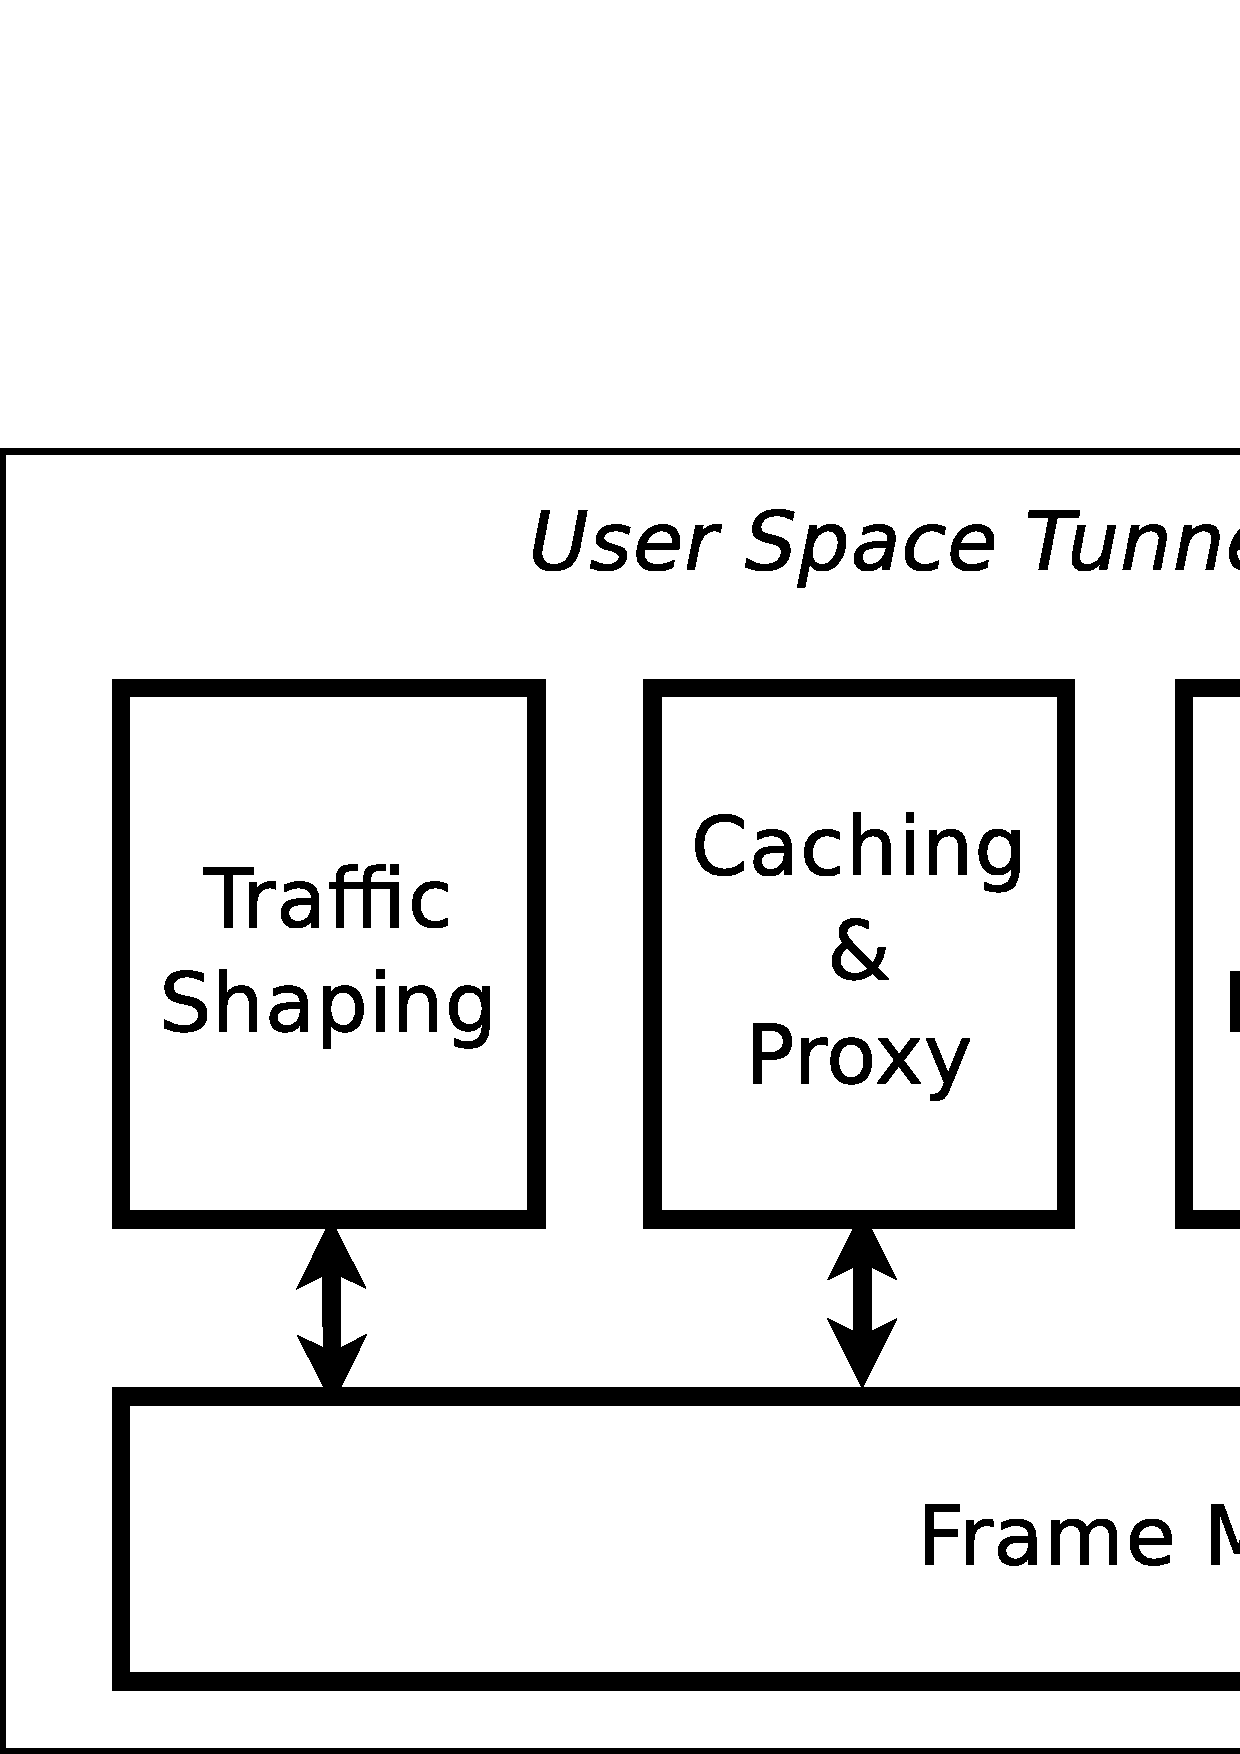
\includegraphics[width=0.6\columnwidth]{figures/TunProc.pdf}
%  \caption{Flow of packets in each \meddle}
%  \label{fig:MeddleboxPacketFlow}
% \end{figure}

\section{Feasibility}
\label{sec:eval}
We now highlight several key questions regarding the feasibility of
deploying our approach at scale. Because our approach in part depends
on users installing a VPN configuration and tunneling all traffic
through \meddle, we evaluate whether the cost to the user in terms
of performance, power and data quota is sufficiently low. 

\noindent\textbf{Power consumption.} Tunneling traffic through a
\meddle requires that all traffic to be encrypted. We observed a 
10\% increase in power consumption when streaming an HD 
video to Android and iPhone devices using our IPsec tunnel. 

\noindent\textbf{Data consumption.} IPsec encapsulation slightly
inflates packet sizes, in addition to preventing carrier middleboxes
from applying their own compression. We measured the overhead of the
tunnel in terms of data overhead from IPsec headers and keepalive
messages, finding that it ranges from 8--12\%. For our measurements we
setup a \meddle as a VPN gateway for an iPhone and Android
phone. On each phone we accessed the Internet using the VPN tunnel for
one hour. Our test traffic was generated by activities that we 
expect to be typical of mobile device usage: Web searches, map
searches, online shopping, downloading popular apps, emailing and
reading the news. We also uploaded a picture to Facebook and Twitter,
streamed a video on YouTube, and played a popular game (Angry Birds).

\noindent\textbf{Performance.} By forcing user traffic to \meddle 
and interposing on flows, we may add latency both due to additional
hops and due to processing time at the \meddle. We envision a
DONAR-style deployment where users are dynamically redirected to a
\meddle based on network conditions and server
load~\cite{wendell:donar}. Given this model, we evaluate whether we
can locate servers near mobile-network egress points using a
deployment such as PlanetLab, and found that this is generally the
case. For this experiment, we used data from approximately 10 mobile
phones located throughout the US and issued traceroutes from the
devices to targets in Google and Facebook's networks. We then used the
first non-private IP address seen from the mobile device on the path
to a server. We assume that this corresponds to the first router
adjacent to the mobile carrier's public Internet egress point. Note
that we could not simply ping the device IPs because mobile carriers
filter inbound ping requests. Using this set of egress adjacencies, we
determined the round-trip time from each PlanetLab site, then took the
average of the nearest five sites to represent the case where a host
at the nearest site is unavailable due to load or other issues. The
average latency to each router was between 3\,ms and 13\,ms, with a
median of 5\,ms. Thus, when compared to RTTs of 10s or 100s of
milliseconds that exist in mobile networks, the additional latencies
from traversing a \meddle is expected to be relatively small or
even negligible.

\section{Incentive for Users}

We do not expect any single incentive to be sufficient for user
adoption of \meddle. Rather, the research enabled by \meddle should
form a positive feedback loop in which new, proven research artifacts
become additional incentives for user adoption, thus enabling further
research.  

For starters, we have implemented a DNS based filter to block ads,
analytics, and mediation sites. Blocking ads is an important incentive
because Vallina-rodriguez \etal~\cite{Vallina-rodriguez:2012:AdCache}
observe that ads account for 5\% of daily traffic from more than 50\%
of Android users in a large European ISP. Our ad blocking engine
relies on publicly available 
list of domains for ads and analytics~\cite{YoyoAds}. To filter
domains specific to mobile networks, we also use the recent research
on mobile ads~\cite{Leontiadis:2012:AdsMobile, hornyack:appfence}. We
have also built a prototype framework inspired by Mozilla
Collusion~\cite{collusion} to generate a graph of domains with which
the mobile device exchanges data. We are currently working on a
frontend to enable users to view this graph.

\section{Conclusion \& Roadmap}

Using overlays for a user based measurement study is not
new~\cite{Joseph:2006:OCALA}; however, to the best of our knowledge, we
are the first to propose and build such a system for mobile clients. 

% \begin{figure}
%   \centering
%   \includegraphics[width=0.7\columnwidth]{figures/OpenSwitch.pdf}
%   \caption{Meddle Server. \emph{Open vSwitch to route packets via
%       VMs. The VMs used depend on the source of the traffic and type
%       of packets.}} 
%   \label{fig:MeddleServer}
% \end{figure}

On each \meddle server, we envision using Open
vSwitch~\cite{Openvswitch} to process packets on Virtual Machines
depending on the source of the traffic and the protocols used to
create the packets~\cite{Sekar:2012:ConsolidatedMBox}. This
architecture enables us to test algorithms for content coalescing,
caching, prefetching, and offloading the work of processing the DOM to
speed up page load times~\cite{silk,opera-mini,google-spdy}.
Furthermore, we envision that most of the interesting opportunities
for mobile offloading will come at the intersection of severe
constraints for mobile devices (power, data volume quota, and
latencies) and the applications that extensively exercise those
constraints. For instance, distributed hash tables (DHTs) are an
example of a distributed service that has become critical for a
variety of applications from P2P communication to content caching and
anonymous networking. Using a split-application model, mobile device
need only send a request for a key to the server-side and the server
can perform all the network operations required to locate the value
without consuming mobile network bandwidth.

\scriptsize
\bibliographystyle{abbrv}
\bibliography{related_work}
\normalsize

\end{document}
